% Formatted for ICFP 2018: ACM Small template
\documentclass[format=acmsmall, review=false, screen=true]{acmart}

%\usepackage{graphicx}
%\usepackage{caption} 
%\usepackage{subcaption}
%\usepackage{hyperref}
%\usepackage{listings}
%\usepackage{hhline}
%\usepackage{float}
%\usepackage{amssymb}
%\usepackage[autostyle=true]{csquotes}
%\usepackage{amsmath}
%\usepackage{marvosym}
\usepackage{minted}

% Metadata Information
% TODO:
\acmJournal{PACMPL}
\acmVolume{9}
\acmNumber{4}
\acmArticle{39}
\acmYear{2018}
\acmMonth{9}
\copyrightyear{2018}
%\acmArticleSeq{9}

% Copyright
%\setcopyright{acmcopyright}	% = copyright transfer to ACM
\setcopyright{acmlicensed} 		% = retaining copyright but granting ACM exclusive publication rights
%\setcopyright{rightsretained}  % = open access on payment of a fee
%\setcopyright{usgov}
%\setcopyright{usgovmixed}
%\setcopyright{cagov}
%\setcopyright{cagovmixed}

% DOI
% TODO
\acmDOI{0000001.0000001}

% Paper history
\received{March 2018}
\received[revised]{March 2018}
\received[accepted]{March 2018}

% Document starts
\begin{document}
% Title portion. Note the short title for running heads
\title[Pure functional epidemics]{Pure functional epidemics}
\subtitle{An Agent-Based Approach}

\author{Jonathan Thaler}
\orcid{TODO}
\email{jonathan.thaler@nottingham.ac.uk}
\author{Thorsten Altenkirch}
\email{thorsten.altenkirch@nottingham.ac.uk}
\author{Peer-Olaf Siebers}
\affiliation{%
  \institution{University of Nottingham}
  \streetaddress{7301 Wollaton Rd}
  \city{Nottingham}
  \postcode{NG8 1BB}
  \country{United Kingdom}}
\email{peer-olaf.siebers@nottingham.ac.uk}

\begin{abstract}
TODO: cite my own 1st paper from SSC2017: add it to citations

TODO: refine it: start with simulating epidemics and then go into ABS

Agent-Based Simulation (ABS) is a methodology in which a system is simulated in a bottom-up approach by modelling the micro interactions of its constituting parts, called agents, out of which the global macro system behaviour emerges. So far, the Haskell community hasn't been much in contact with the community of ABS due to the latter's primary focus on the object-oriented programming paradigm. This paper tries to bridge the gap between those two communities by introducing the Haskell community to the concepts of ABS. We do this by deriving an agent-based implementation for the simple SIR model from epidemiology. In our approach we leverage the basic concepts of ABS with functional reactive programming from Yampa and Dunai which results in a surprisingly fresh, powerful and convenient EDSL for programming ABS in Haskell.
\end{abstract}

%
% The code below should be generated by the tool at
% http://dl.acm.org/ccs.cfm
% Please copy and paste the code instead of the example below.
%
% TODO needs to be generated
%\begin{CCSXML}
%<ccs2012>
% <concept>
%  <concept_id>10010520.10010553.10010562</concept_id>
%  <concept_desc>Computer systems organization~Embedded systems</concept_desc>
%  <concept_significance>500</concept_significance>
% </concept>
% <concept>
%  <concept_id>10010520.10010575.10010755</concept_id>
%  <concept_desc>Computer systems organization~Redundancy</concept_desc>
%  <concept_significance>300</concept_significance>
% </concept>
% <concept>
%  <concept_id>10010520.10010553.10010554</concept_id>
%  <concept_desc>Computer systems organization~Robotics</concept_desc>
%  <concept_significance>100</concept_significance>
% </concept>
% <concept>
%  <concept_id>10003033.10003083.10003095</concept_id>
%  <concept_desc>Networks~Network reliability</concept_desc>
%  <concept_significance>100</concept_significance>
% </concept>
%</ccs2012>
%\end{CCSXML}
%
%\ccsdesc[500]{Computer systems organization~Embedded systems}
%\ccsdesc[300]{Computer systems organization~Redundancy}
%\ccsdesc{Computer systems organization~Robotics}
%\ccsdesc[100]{Networks~Network reliability}

%
% End generated code
%

\keywords{Haskell, Functional Programming, Functional Reactive Programming, Agent-Based Simulation}

\maketitle

\section{Introduction}
There exists a large number of simulation packages which allow the convenient creation of System Dynamics simulations by straight-forward visual diagram creation. One simply creates stocks and flows, connects them, specifies the flow-rates and initial parameters and then runs the model. An example for such a visual diagram creation in the simulation package AnyLogic can be seen in Figure \ref{fig:sir_stockflow_diagram}.

\begin{figure}
	\centering
	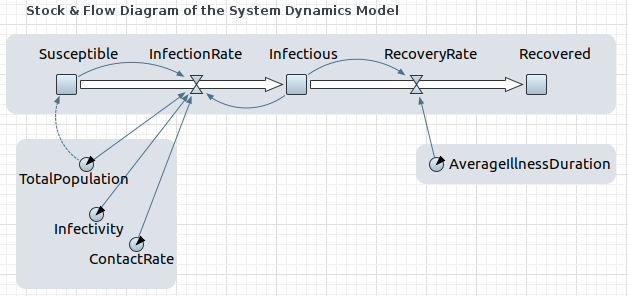
\includegraphics[width=.5\textwidth, angle=0]{./fig/SIR_SD_STOCKFLOW_DIAGRAMM.png}
	\caption{Visual System Dynamics Diagram of the SIR model in AnyLogic Personal Learning Edition 8.3.1.}
	\label{fig:sir_stockflow_diagram}
\end{figure}

Still, implementing System Dynamics directly in code is not as straight forward and involves numerical integration which can be quite tricky to get right. Thus, the aim of this paper is to look into how System Dynamics models can be implemented in code correctly without the use of a simulation package. We use the well known SIR model \cite{kermack_contribution_1927} from epidemiology to demonstrate our approach.

Our language of choice is Haskell because it emphasises a declarative programming style in which one describes \textit{what} instead of \textit{how} to compute. Further it allows to rule out interference with non-deterministic influences or side-effects already at compile-time. This is of fundamental importance for System Dynamics because it behaves completely deterministic and involves no stochastics or non-determinism whatsoever. Also, we make use of Functional Reactive Programming which allows to express continuous-time systems in a functional way. 

We show that by this approach we can arrive at correct-by-construction implementations of System Dynamic models. This means that the correctness of the code is obvious because we have closed the gap between the model specification and its implementation. Thus, the contribution of the paper is the demonstration of how to implement correct-by-construction System Dynamics simulations using Haskell and Functional Reactive Programming.

\section{Defining Agent-Based Simulation}
\label{sec:defining_abs}

Agent-Based Simulation (ABS) is a methodology to model and simulate a system where the global behaviour may be unknown but the behaviour and interactions of the parts making up the system is of knowledge. Those parts, called agents, are modelled and simulated out of which then the aggregate global behaviour of the whole system emerges. So the central aspect of ABS is the concept of an agent which can be understood as a metaphor for a pro-active unit, situated in an environment, able to spawn new agents and interacting with other agents in some neighbourhood by exchange of messages. 
We informally assume the following about our agents \cite{siebers_introduction_2008}, \cite{wooldridge_introduction_2009}, \cite{siebers_discrete-event_2010}, \cite{dawson_opening_2014}, \cite{macal_everything_2016}:

\begin{itemize}
	\item They are uniquely addressable entities with some internal state over which they have full, exclusive control.
	\item They are pro-active which means they can initiate actions on their own e.g. change their internal state, send messages, create new agents, terminate themselves.
	\item They are situated in an environment and can interact with it.
	\item They can interact with other agents which are situated in the same environment by means of messaging.
\end{itemize} 

\begin{comment}
Epstein \cite{epstein_generative_2012} identifies ABS to be especially applicable for analysing \textit{"spatially distributed systems of heterogeneous autonomous actors with bounded information and computing capacity"}. %Thus in the line of the established simulation methodologies (see Table \ref{tab:simulation_types}), ABS is the most powerful one as listed in :
It exhibits the following properties:

\begin{itemize}
	\item Linearity \& Non-Linearity - actions of agents can lead to non-linear behaviour of the system.
	\item Time - agents act over time which is also the source of their pro-activity.
	\item States - agents encapsulate some state which can be accessed and changed during the simulation.
	\item Feedback-Loops - because agents act continuously and their actions influence each other and themselves in subsequent time-steps, feedback-loops are the norm in ABS. 
	\item Heterogeneity - although agents can have same properties like height, sex,... the actual values can vary arbitrarily between agents.
	\item Interactions - agents can be modelled after interactions with an environment or other agents. %, making this a unique feature of ABS, not possible in the other simulation models.
	\item Spatiality \& Networks - agents can be situated within e.g. a spatial (discrete 2D, continuous 3D,...) or complex network environment. % making this also a unique feature of ABS, not possible in the other simulation models.
\end{itemize}
\end{comment}

\begin{comment}
Note that there doesn't exist a commonly agreed technical definition of ABS but the field draws inspiration from the closely related field of Multi-Agent Systems (MAS) \cite{wooldridge_introduction_2009}, \cite{weiss_multiagent_2013}. It is important to understand that MAS and ABS are two different fields where in MAS the focus is much more on technical details, implementing a system of interacting intelligent agents within a highly complex environment with the focus primarily on solving AI problems.
\end{comment}

\section{The SIR Model}
To explain the concepts of ABS and of our functional reactive approach to it, we introduce the SIR model as a motivating example. The SIR model is a a very well studied and understood compartment model from epidemiology which allows to simulate the dynamics of an infectious disease spreading through a population. In this model, people in a population of size $N$ can be in either one of three states \textit{Susceptible}, \textit{Infected} or \textit{Recovered} at a particular time, where it is assumed that initially there is at least one infected person in the population. People interact with each other \textit{on average} with a given rate $\beta$ per time-unit and get infected with a given probability $\gamma$ when interacting with an infected person. When infected, a person recovers \textit{on average} after $\delta$ time-units and is then immune to further infections. An infected person interaction with another infected one is never re-infected, thus interactions amongst infected people is not important in this model. This definition gives rise to three compartments with the transitions as seen in Figure \ref{fig:sir_transitions}.

\begin{figure}
	\centering
	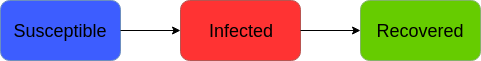
\includegraphics[width=.4\textwidth, angle=0]{./fig/SIR_transitions.png}
	\caption{Transitions in the SIR compartment model.}
	\label{fig:sir_transitions}
\end{figure}

The dynamics of this model over time can be formalized using the following equations:

$\frac{\mathrm d S}{\mathrm d t} = -infectionRate$ \\
$\frac{\mathrm d I}{\mathrm d t} = infectionRate - recoveryRate$ \\
$\frac{\mathrm d R}{\mathrm d t} = recoveryRate$ \\

$infectionRate = \frac{I \beta S \gamma}{N}$ \\
$recoveryRate = \frac{I}{\delta}$ \\

Solving these can be done using the System-Dynamics (SD) approach which solves the equations by integrating over time. In the SD terminology, the intergrals are called \textit{Stocks} and the values over which is integrated over time are called \textit{Flows}.

$S(t) = N + \int_0^t -infectionRate\, \mathrm{d}t$ \\
$I(t) = 1 + \int_0^t infectionRate - recoveryRate\, \mathrm{d}t$ \\
$R(t) = \int_0^t recoveryRate\, \mathrm{d}t$ \\

There exist a huge number of software-packages which allow to conveniently express SD models using a visual approach like in Figure \ref{fig:sir_sd_stockflow_diagramm}.

\begin{figure}
	\centering
	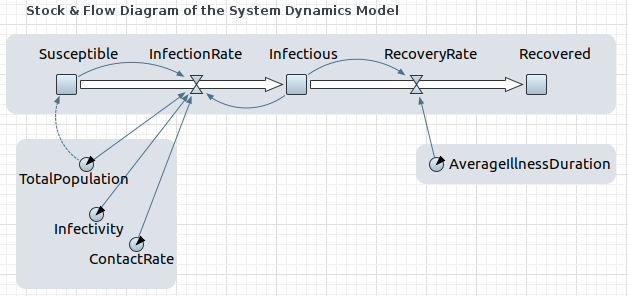
\includegraphics[width=.4\textwidth, angle=0]{./fig/SIR_SD_STOCKFLOW_DIAGRAMM.png}
	\caption{A visual representation of the stocks and flows in the SIR compartment model (Image courtesy of AnyLogic Company).}
	\label{fig:sir_sd_stockflow_diagramm}
\end{figure}

Running the SD simulation over time results in the dynamics as shown in Figure \ref{fig:sir_sd_dynamics_anylogic} with the given variables.

\begin{figure}
	\centering
	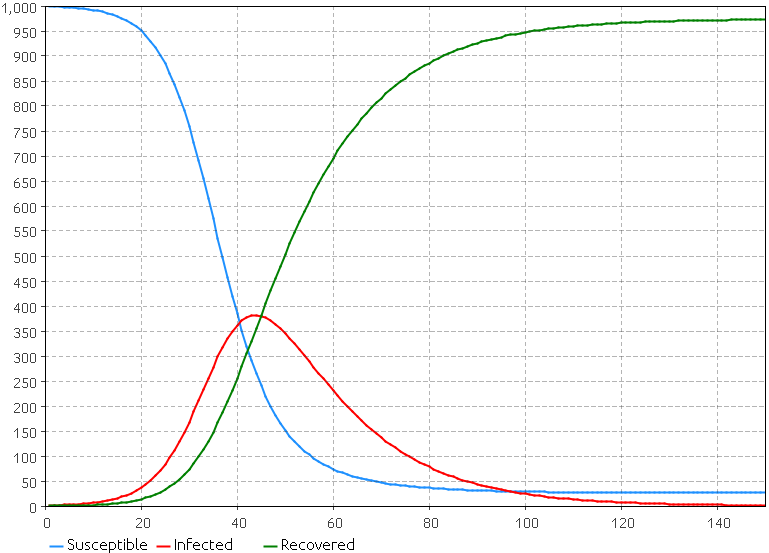
\includegraphics[width=.4\textwidth, angle=0]{./fig/SIR_SD_DYNAMICS_ANYLOGIC.png}
	\caption{Dynamics of the SIR compartment model using the System Dynamics approach generated with the AnyLogic Personal Learning Edition 8.1.0. Population Size $N$ = 1000, contact rate $\beta = 1/5$, infection probability $\gamma = 0.05$, illness duration $\delta = 15$.}
	\label{fig:sir_sd_dynamics_anylogic}
\end{figure}

\subsection{An Agent-Based approach}
The SD approach is inherently Top-Down because the emergent property of the system is formalized in differential equations. The question is if such a top-down behaviour can be emulated using ABS, which is inherently bottom-up. Also the question is if there are fundamental drawbacks and benefits when doing so using ABS. Indeed such questions were asked before and modelling the SD approach of the SIR model is possible using an agent-based approach. It is important to note that SD treats the population completely continuous which results in non-discrete values of stocks e.g. 3.1415 infected persons. Thus the fundamental approach to map the SIR model to an ABS is to discretisize the population and model each person in the population as an invidivual agent. The transition  between the states are no longer happening according to continuous differential equations but due to discrete events caused both by interactions amongst the agents and time-outs. The behaviour can be defined as follows:

\begin{itemize}
	\item Every agent makes on average contact with $\beta$ random other agents per time unit. In ABS we can only contact discrete agents thus we model this by generating a random event on average every $\beta$ time units.
	
	\item An agent does not know the other agents state when making contact with it, thus we need a mechanism in which agents reveal their state in which they are in \textit{at the moment of making contact}. Obviously the already mentioned messaging-mechanism which allows agents to interact is perfectly suited to do this.
	\begin{itemize}
		\item \textit{Susceptible} agent: sends a "Susceptible" message when contacting another agent. There is no need to reply to other incoming messages as making contact with a susceptible agent has no influence on the state of an agent.
		\item \textit{Infected} agent: sends a "Infected" message when contacting another agent. An infected agent now needs to reply to incoming "Susceptible" messages with an "Infected" message to let the susceptible agent know that it has made contact with an infected agent.
		\item \textit{Recovered} agent: does not need to send messages because contacting it or being contacted by it has no influence on the state.
	\end{itemize}
	
	\item Susceptible to Infected: needs to have made contact with an infected agent which happens when it receives an "Infected" message. If this occurs an infection occurs with a probability of $\gamma$. The infection can be calculated by drawing from a uniform random-distribution between 0 and 1 and comparing the value to $\gamma$, if the drawn value $p < \gamma$ then infection occurs. Note that this needs to be done for \textit{every} received "Infected" message.
	
	\item Infected to Recovered: a person recovers \textit{on average} after $\delta$ time unites. This is implemented by drawing the duration from an exponential distribution (TODO: borchschev) with $\lambda = \frac{1}{\delta}$ and making the transition after this duration.
\end{itemize}

We will discuss the implementation of this approach in the following sections and as will be shown FrABS will allow us to express this behaviour very explicitly looking very much like a formal ABS specification of the problem. For now we will give the resulting dynamics in Figure TODO

TODO: how many initially infected agents? one should be enough, at least in my implementation

TODO: 100 vs. 1000 vs. 5.000 agents

TODO: problem in my code: need exponentially occasionally not uniform distributed! => OK, occasionally draws from exponential-distribution
TODO: what differences do the different update strategies make?

\subsection{Blub}
TODO: It should be possible to formally show that spatial SIR and WildFire are the same model. NOTE: they are NOT the same, the fundamental difference is that in the WildFire model only the burning cells initiate the ignition - if we compare this to the SIR, the burning cells would be infected agents and although in the spatial SIR model the infected agents make contact with other agents, so do the susceptible ones which does NOT occur in wildfire

TODO: cite my own work on update-strategies

TODO: can we formally show that the SIR approximates the SD model?

TODO: cite papers which discuss how to approximate a SD model by ABS
- Macal (2010) - To Agent-Based Simulation From System Dynamics 
	-> i am very unhappy with this paper: first it does not give concrete parameters for the SD model so it is impossible to replicate. Also i think it has a systematical error as the infected agents make no contact but this is required as evident from the SD-models infection-rate which also incorporates. TODO: write an email to this guy: why are the infectious not contacting the other agents? this seems to be a systematical error
- Borshchev, Filippov (2004) - From System Dynamics and Discrete Event to Practical Agent Based Modeling: Reasons, Techniques, Tools
	-> its VERY IMPORTANT point is that we need to draw the illness-duration from an exponential-distribution because the illness-duration is proportional to the size of the infected. note: this is wrongly expressed, need to find the correct formulation

		-> my emulation of SD using ABS is really an implementation of the SD model and follows it - they are equivalent
		-> my ABS implementation is the same as / equivalent to the SD emulation
			=> thus if i can show that my SD emulation is equlas to the SD model
			=> AND that the ABS implementation is the same as the SD emulation
			=> THEN the ABS implementation is an SD implementation, and we have shown this in code for the first time in ABS
			


\section{Deriving a pure functional approach}
\label{sec:functional_approach}

We presented a high-level agent-based approach to the SIR model in the previous section, which focused only on the states and the transitions, but we haven't talked about technical implementation. 

In \cite{thaler_art_2017} two fundamental problems of implementing an agent-based simulation from a programming-language agnostic point of view is discussed. The first problem is how agents can be pro-active and the second how interactions and communication between agents can happen. For agents to be pro-active, they must be able to perceive the passing of time, which means there must be a concept of an agent-process which executes over time. Interactions between agents can be reduced to the problem of how an agent can expose information about its internal state which can be perceived by other agents. Further the authors have shown the influence of different deterministic and non-deterministic elements in agent-based simulation on the dynamics and how the influence of non-determinism can completely break them down or result in different dynamics despite same initial conditions. This means that we want to rule out any potential source of non-determinism.

\begin{figure}
	\centering
	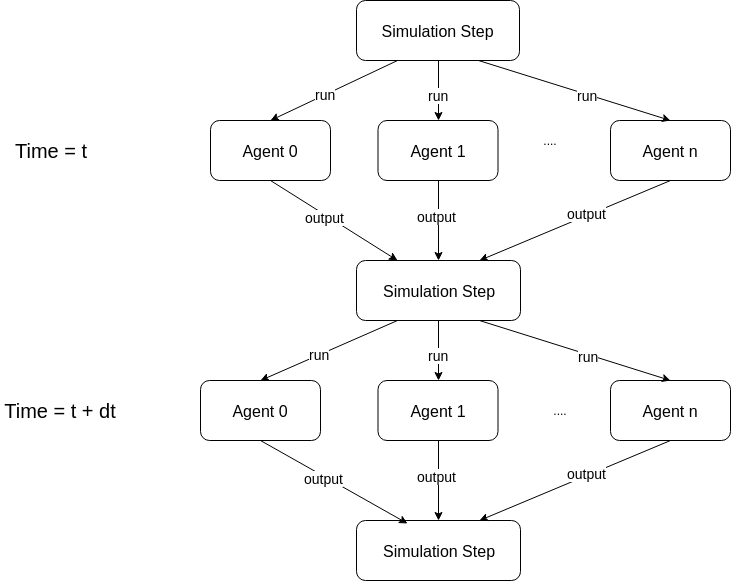
\includegraphics[width=.4\textwidth, angle=0]{./fig/diagrams/parallel_strategy.png}
	\caption{Running the agents (conceptually) in parallel lock-step. All agents observe the same environment state during a step and run isolated from each other - changes made by an agent to the environment is only visible in the next one.}
	\label{fig:parallel_strategy}
\end{figure}

In this section we will derive a pure functional approach for an agent-based simulation of the SIR model in which we will pose solutions to the previously mentioned problems. We will start out with a straight forward approach in Yampa and show its limitations. Then in further steps we will add more concepts and generalisations, ending up at the final approach which utilises Monadic Stream Functions, a generalisation of FRP.

Of paramount importance is to keep our implementations pure which rules out the use of the IO Monad and thus any potential source of non-determinism under all circumstances because we would loose all compile time guarantees about reproducibility. Still we will make use of the Random and State Monad which indeed allow side-effects but the crucial point here is that we restrict side-effects only to these types in a controlled way without allowing general unrestricted effects
\footnote{The code of all steps can be accessed freely through the following URL: \url{https://github.com/thalerjonathan/phd/tree/master/public/purefunctionalepidemics/code}}.

TODO: a general functional ABS interface: agentstate -> world > agentstate and a function world -> [agentstate] -> world

TODO: sequential is wrong semantics because all agents act at the sa.e time, if we impose an ordering it could be the case that e.g. the infection spreads from top left corner to bottom right but not the other way round. for many ab models which run sequentially the established approach is thus to shuffle the agents in each step to avoid these kind of semantic problems. In FP we can enforce such an iteation strategy already in the types. the flaw reflects exactly my iterating paper message: the strategy needs to reflect the semantics of the model

TODO: make clear that ABS often runs agents sequentially and shuffles them. there is no agreed "true" way as we have shown as itvresults in different semantics but in  functional programming the parallel approach is the best fit. and for SIR its the only correct one

TODO: problem of switch, dSwitch won't help: the next SF is always applied immediately!, need a notYet

TODO: next steps: when we have conflicts in Environment e.g. moving agents where only a single one can occupy a cell then we need some conflict resolving: FRP allows to re-run old versions of sf/msf as long as the underlying monad is robust to that which the random monad is

TODO: benefit of functional programming: we can have 'sequential' monadic effectful behaviour but then enforce through the type a read-only shared environment which results in a "parallel" update strategy.

TODO: emphasise the different semantics of sequential iteration and cite my iterating paper 

TODO: re-do Performance runs in BOTH papers

SPACE: reduce supersampling: dont provide yampa function
SPACE: compress the step to msfs into adding Environment
SPACE: shorten MSF example in Background
SPACE: reduce code in paper as well in last step because hardly necessary anymore

\subsection{Functional Reactive Programming}
\label{sec:step2_frp}
As described in the Section \ref{sec:back_frp}, Arrowized FRP \cite{hughes_generalising_2000} is a way to implement systems  with continuous and discrete time-semantics where the central concept is the Signal Function, which can be understood as a process over time, mapping an input- to an output-signal. Technically speaking, a signal function is a continuation which allows to capture state using closures and hides away the $\Delta t$ which means that it is never exposed explicitly to the programmer, meaning it cannot be messed with.

The concept of processes over time is an ideal match for our agents and our system as a whole thus we will implement them and the whole system as signal functions.

\subsubsection{Implementation}
We start by defining the SIR states as ADTs and our agents as signal function (SF) which receives the SIR states of all agents as input and outputs the current SIR state of the agent:

\begin{HaskellCode}
data SIRState = Susceptible | Infected | Recovered

type SIRAgent = SF [SIRState] SIRState 
\end{HaskellCode}

Now we can define the behaviour of an agent to be the following:

\begin{HaskellCode}
sirAgent :: RandomGen g => g -> SIRState -> SIRAgent
sirAgent g Susceptible = susceptibleAgent g
sirAgent g Infected    = infectedAgent g
sirAgent _ Recovered   = recoveredAgent
\end{HaskellCode}

Depending on the initial state we return the corresponding behaviour. Note that we are passing a random-number generator instead of running in the Random Monad because signal functions as implemented in Yampa are not capable of being monadic. 

We see that the recovered agent ignores the random-number generator because a recovered agent does nothing, stays immune forever and can not get infected again in this model. Thus a recovered agent is a consuming state from which there is no escape, it simply acts as a sink which returns constantly \textit{Recovered}:

\begin{HaskellCode}
recoveredAgent :: SIRAgent
recoveredAgent = arr (const Recovered)
\end{HaskellCode}

Lets look how we can implement the behaviour of a susceptible agent. It makes contact \textit{on average} with $\beta$ other random agents. For every \textit{infected} agent it gets into contact with, it becomes infected with a probability of $\gamma$. If an infection happens, it makes the transition to the \textit{Infected} state. To make contact, it gets fed the states of all agents in the system from the previous time-step so it can draw random contacts - this is one, very naive way of implementing the interactions between agents.

Thus a susceptible agent behaves as susceptible until it becomes infected. Upon infection an \textit{Event} is returned which results in switching into the \textit{infectedAgent} SF, which causes the agent to behave as an infected agent from that moment on. When an infection event occurs we change the behaviour of an agent using the Yampa combinator \textit{switch}, which is quite elegant and expressive as it makes the change of behaviour at the occurrence of an event explicit. Note that to make contact \textit{on average}, we use Yampas \textit{occasionally} function which requires us to carefully select the right $\Delta t$ for sampling the system as will be shown in results. 

%\begin{samepage}
\begin{HaskellCode}
susceptibleAgent :: RandomGen g => g -> SIRAgent
susceptibleAgent g = 
    switch (susceptible g) (const (infectedAgent g))
  where
    susceptible :: RandomGen g 
      => g -> SF [SIRState] (SIRState, Event ())
    susceptible g = proc as -> do
      makeContact <- occasionally g (1 / contactRate) () -< ()
      if isEvent makeContact
        then (do
          -- draw random element from the list
          a <- drawRandomElemSF g -< as
          case a of
            Infected -> do
              -- returns True with given probability
              i <- randomBoolSF g infectivity -< ()
              if i
                then returnA -< (Infected, Event ())
                else returnA -< (Susceptible, NoEvent)
             _       -> returnA -< (Susceptible, NoEvent))
        else returnA -< (Susceptible, NoEvent)
\end{HaskellCode}
%\end{samepage}

To deal with randomness in an FRP way we implemented additional signal functions built on the \textit{noiseR} function provided by Yampa. This is an example for the stream character and statefulness of a signal function as it allows to keep track of the changed random-number generator internally through the use of continuations and closures. Here we provide the implementation of \textit{randomBoolSF}. \textit{drawRandomElemSF} works similar but takes a list as input and returns a randomly chosen element from it:

\begin{HaskellCode}
randomBoolSF :: RandomGen g => g -> Double -> SF () Bool
randomBoolSF g p = proc _ -> do
  r <- noiseR ((0, 1) :: (Double, Double)) g -< ()
  returnA -< (r <= p)
\end{HaskellCode}

An infected agent recovers \textit{on average} after $\delta$ time units. This is implemented by drawing the duration from an exponential distribution \cite{borshchev_system_2004} with $\lambda = \frac{1}{\delta}$ and making the transition to the \textit{Recovered} state after this duration. Thus the infected agent behaves as infected until it recovers, on average after the illness duration, after which it behaves as a recovered agent by switching into \textit{recoveredAgent}. As in the case of the susceptible agent, we use the \textit{occasionally} function to generate the event when the agent recovers. Note that the infected agent ignores the states of the other agents as its behaviour is completely independent of them.

\begin{HaskellCode}
infectedAgent :: RandomGen g => g -> SIRAgent
infectedAgent g = switch infected (const recoveredAgent)
  where
    infected :: SF [SIRState] (SIRState, Event ())
    infected = proc _ -> do
      recEvt <- occasionally g illnessDuration () -< ()
      let a = event Infected (const Recovered) recEvt
      returnA -< (a, recEvt)
\end{HaskellCode}

For running the simulation we use Yampas function \textit{embed}:

\begin{HaskellCode}
runSimulation :: RandomGen g 
  => g -> Time -> DTime -> [SIRState] -> [[SIRState]]
runSimulation g t dt as 
    = embed (stepSimulation sfs as) ((), dts)
  where
    steps     = floor (t / dt)
    dts       = replicate steps (dt, Nothing)
    n         = length as
    (rngs, _) = rngSplits g n [] -- unique rngs for each agent
    sfs       = zipWith sirAgent rngs as
\end{HaskellCode}

What we need to implement next is a closed feedback-loop - the heart of every agent-based simulation. Fortunately, \cite{nilsson_functional_2002, courtney_yampa_2003} discusses implementing this in Yampa. The function \textit{stepSimulation} is an implementation of such a closed feedback-loop. It takes the current signal functions and states of all agents, runs them all in parallel and returns this step's new agent states. Note the use of \textit{notYet} which is required because in Yampa switching occurs immediately at $t = 0$. If we don't delay the switching at $t = 0$ until the next step, we would enter an infinite switching loop - \textit{notYet} simply delays the first switching until the next time-step.

\begin{HaskellCode}
stepSimulation :: [SIRAgent] -> [SIRState] -> SF () [SIRState]
stepSimulation sfs as =
    dpSwitch
      -- feeding the agent states to each SF
      (\_ sfs' -> (map (\sf -> (as, sf)) sfs'))
      -- the signal functions
      sfs
      -- switching event, ignored at t = 0         
      (switchingEvt >>> notYet)
      -- recursively switch back into stepSimulation         
      stepSimulation                            
  where
    switchingEvt :: SF ((), [SIRState]) (Event [SIRState])
    switchingEvt = arr (\ (_, newAs) -> Event newAs)
\end{HaskellCode}

Yampa provides the \textit{dpSwitch} combinator for running signal functions in parallel, which has the following type-signature:

\begin{HaskellCode}
dpSwitch :: Functor col
         -- routing function
         => (forall sf. a -> col sf -> col (b, sf))
         -- SF collection
         -> col (SF b c)
         -- SF generating switching event     
         -> SF (a, col c) (Event d)
         -- continuation to invoke upon event           
         -> (col (SF b c) -> d -> SF a (col c))
         -> SF a (col c)
\end{HaskellCode}

Its first argument is the pairing-function which pairs up the input to the signal functions - it has to preserve the structure of the signal function collection. The second argument is the collection of signal functions to run. The third argument is a signal function generating the switching event. The last argument is a function which generates the continuation after the switching event has occurred. \textit{dpSwitch} returns a new signal function which runs all the signal functions in parallel and switches into the continuation when the switching event occurs. The d in \textit{dpSwitch} stands for decoupled which guarantees that it delays the switching until the next time-step: the function into which we switch is only applied in the next step, which prevents an infinite loop if we switch into a recursive continuation.

Conceptually, \textit{dpSwitch} allows us to recursively switch back into the \textit{stepSimulation} with the continuations and new states of all the agents after they were run in parallel. 

\subsubsection{Results}
The dynamics generated by this step can be seen in Figure \ref{fig:sir_abs_dynamics_frp}. 

\begin{figure}
\begin{center}
	\begin{tabular}{c c}
		\begin{subfigure}[b]{0.22\textwidth}
			\centering
			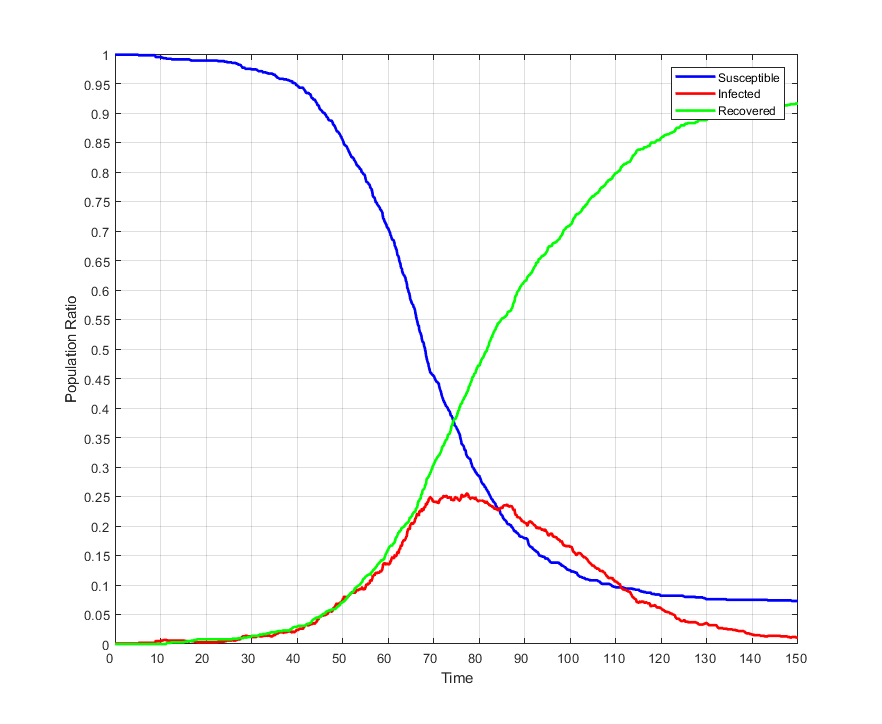
\includegraphics[width=1\textwidth, angle=0]{./fig/step2_yampa/SIR_1000agents_150t_01dt.png}
			\caption{$\Delta t = 0.1$}
			\label{fig:sir_abs_approximating_01dt_1000agents}
		\end{subfigure}
		
		&
    	
		\begin{subfigure}[b]{0.22\textwidth}
			\centering
			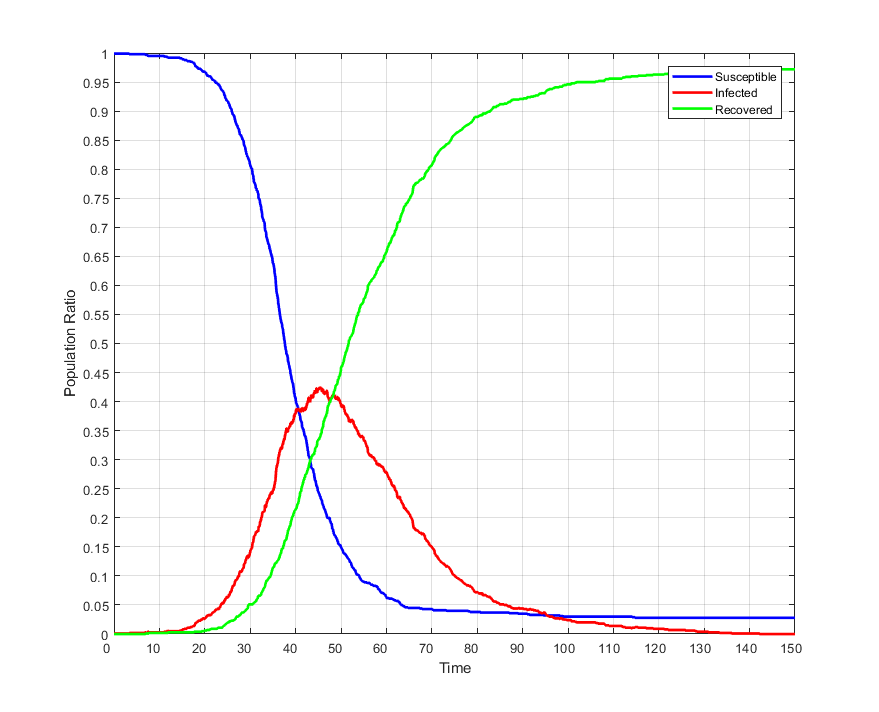
\includegraphics[width=1\textwidth, angle=0]{./fig/step2_yampa/SIR_1000agents_150t_001dt.png}
			\caption{$\Delta t = 0.01$}
			\label{fig:sir_abs_approximating_001dt_1000agents}
		\end{subfigure}
	\end{tabular}
	
	\caption{FRP simulation of agent-based SIR showing the influence of different $\Delta t$. Population size of 1,000 with contact rate $\beta = \frac{1}{5}$, infection probability $\gamma = 0.05$, illness duration $\delta = 15$ with initially 1 infected agent. Simulation run for 150 time-steps with respective $\Delta t$.} 
	\label{fig:sir_abs_dynamics_frp}
\end{center}
\end{figure}

By following the FRP approach we assume a continuous flow of time which means that we need to select a \textit{correct} $\Delta t$ otherwise we would end up with wrong dynamics. The selection of a correct $\Delta t$ depends in our case on \textit{occasionally} in the \textit{susceptible} behaviour, which randomly generates an event on average with \textit{contact rate} following the exponential distribution. To arrive at the correct dynamics, this requires us to sample \textit{occasionally}, and thus the whole system, with small enough $\Delta t$ which matches the frequency of events generated by \textit{contact rate}. If we choose a too large $\Delta t$, we loose events which will result in wrong dynamics as can be seen in Figure \ref{fig:sir_abs_approximating_01dt_1000agents}. This issue is known as under-sampling and is described in Figure \ref{fig:sampling_issue}.

\begin{figure}
\begin{center}
	\begin{tabular}{c}
		\begin{subfigure}[b]{0.3\textwidth}
			\centering
			
\includegraphics[width=1\textwidth, angle=0]{./fig/diagrams/Undersampling.png}
			\caption{Under-sampling}
			\label{fig:undersampling}
		\end{subfigure}
		
		\\
		
		\begin{subfigure}[b]{0.3\textwidth}
			\centering
			
\includegraphics[width=1\textwidth, angle=0]{./fig/diagrams/Supersampling.png}
			\caption{Super-sampling}
			\label{fig:supersampling}
		\end{subfigure}
	\end{tabular}
	
	\caption{A visual explanation of under-sampling and super-sampling. The black dots represent the time-steps of the simulation. The red dots represent virtual events which occur at specific points in continuous time. In the case of under-sampling, 3 events occur in between the two time steps but \textit{occasionally} only captures the first one. By increasing the sampling frequency either through a smaller $\Delta t$ or super-sampling all 3 events can be captured.} 
	\label{fig:sampling_issue}
\end{center}
\end{figure}

For tackling this issue we have two options. The first one is to use a smaller $\Delta t$ as can be seen \ref{fig:sir_abs_approximating_001dt_1000agents}, which results in the whole system being sampled more often, thus reducing performance. The other option is to implement super-sampling and apply it to \textit{occasionally} which would allow us to run the whole simulation with $\Delta t = 1.0$ and only sample the \textit{occasionally} function with a much higher frequency.

An approach to super-sampling would be to introduce a new combinator to Yampa which allows us to super-sample other signal functions. 

\begin{HaskellCode}
superSampling :: Int -> SF a b -> SF a [b]
\end{HaskellCode}

It evaluates the \textit{SF} argument for \textit{n} times, each with $\Delta t = \frac{\Delta t}{n}$ and the same input argument \textit{a} for all \textit{n} evaluations. At time 0 no super-sampling is performed and just a single output of the \textit{SF} argument is calculated. A list of \textit{b} is returned with length of \textit{n} containing the result of the \textit{n} evaluations of the \textit{SF} argument. If 0 or less super samples are requested exactly one is calculated. We could then wrap the occasionally function which would then generate a list of events. We have investigated super-sampling more in-depth but have to omit this due to lack of space.

\subsubsection{Discussion}
We can conclude that our first step already introduced most of the fundamental concepts of ABS:
\begin{itemize}
	\item Time - the simulation occurs over virtual time which is modelled explicitly divided into \textit{fixed} $\Delta t$ where at each step all agents are executed.
	\item Agents - we implement each agent as an individual, with the behaviour depending on its state.
	\item Feedback - the output state of the agent in the current time-step $t$ is the input state for the next time-step $t + \Delta t$.
	\item Environment - as environment we implicitly assume a fully-connected network (complete graph) where every agent 'knows' every other agent, including itself and thus can make contact with all of them.
	\item Stochasticity - it is an inherently stochastic simulation, which is indicated by the random-number generator and the usage of \textit{occasionally}, \textit{randomBoolSF} and \textit{drawRandomElemSF}.
	\item Deterministic - repeated runs with the same initial random-number generator result in same dynamics. This may not come as a surprise but in Haskell we can guarantee that property statically already at compile time because our simulation runs \textit{not} in the IO Monad. This guarantees that no external, uncontrollable sources of non-determinism can interfere with the simulation.
\end{itemize}

Using FRP in the instance of Yampa results in clarity, expressivity and robustness of our implementation. State is implicitly encoded, depending on which signal function is active. By using explicit time-semantics with \textit{occasionally} we can achieve extremely fine grained stochastics by sampling the system with small $\Delta t$: we are treating it as a truly continuous time-driven agent-based system.

A very severe problem, very hard to find with testing but detectable with in-depth validation analysis, is the fact that in the \textit{susceptible} agent the same random-number generator is used in \textit{occasionally}, \textit{drawRandomElemSF} and \textit{randomBoolSF}. This means that all three stochastic functions, which should be independent from each other, are inherently correlated. This is something one wants to prevent under all circumstances in a simulation, as it can invalidate the dynamics on a very subtle level, and indeed we have tested the influence of the correlation in this example and it has an impact. We left this severe bug in for explanatory reasons, as it shows an example where functional programming actually encourages very subtle bugs if one is not careful. A possible solution would be to simply split the initial random-number generator in \textit{sirAgent} three times (using one of the splited generators for the next split) and pass three random-number generators to \textit{susceptible}.

So far we have an acceptable implementation of an agent-based SIR approach. What we are lacking at the moment is a general treatment of an environment. To conveniently introduce it we want to make use of monads which is not possible using Yampa. In the next step we make the transition to Monadic Stream Functions as introduced in Dunai \cite{perez_functional_2016} which allows FRP within a monadic context.

\subsection{Generalising to Monadic Stream Functions}
\label{sec:generalising_msfs}
A part of the library Dunai is BearRiver, a wrapper which re-implements Yampa on top of Dunai, which should allow us to easily replace Yampa with MSFs. This will enable us to run arbitrary monadic computations in a signal function, solving our problem of correlated random numbers through the use of the Random Monad.

\subsubsection{Identity Monad}
We start by making the transition to BearRiver by simply replacing Yampas signal function by BearRivers', which is the same but takes an additional type parameter \textit{m}, indicating the monadic context. If we replace this type-parameter with the Identity Monad, we should be able to keep the code exactly the same, because BearRiver re-implements all necessary functions we are using from Yampa. We simply re-define the agent signal function, introducing the monad stack our SIR implementation runs in:

\begin{HaskellCode}
type SIRMonad = Identity
type SIRAgent = SF SIRMonad [SIRState] SIRState
\end{HaskellCode}

\subsubsection{Random Monad}
Using the Identity Monad does not gain us anything but it is a first step towards a more general solution. Our next step is to replace the Identity Monad by the Random Monad, which will allow us to run the whole simulation within the Random Monad with the full features of FRP, finally solving the problem of correlated random numbers in an elegant way. We start by re-defining the SIRMonad and SIRAgent:

\begin{HaskellCode}
type SIRMonad g = Rand g
type SIRAgent g = SF (SIRMonad g) [SIRState] SIRState
\end{HaskellCode}

The question is now how to access this Random Monad functionality within the MSF context. For the function \textit{occasionally}, there exists a monadic pendant \textit{occasionallyM} which requires a MonadRandom type-class. Because we are now running within a MonadRandom instance we simply replace \textit{occasionally} with \textit{occasionallyM}. 

\begin{HaskellCode}
occasionallyM :: MonadRandom m => Time -> b -> SF m a (Event b)
-- can be used through the use of arrM and lift
randomBoolM :: RandomGen g => Double -> Rand g Bool
-- this can be used directly as a SF with the arrow notation
drawRandomElemSF :: MonadRandom m => SF m [a] a
\end{HaskellCode}

\subsubsection{Discussion} 
Running in the Random Monad solved the problem of correlated random numbers and elegantly guarantees us that we won't have correlated stochastics as discussed in the previous section. In the next step we introduce the concept of an explicit discrete 2D environment.

\subsection{Adding an environment}
\label{sec:adding_env}
So far we have implicitly assumed a fully connected network amongst agents, where each agent can see and 'knows' every other agent. This is a valid environment and in accordance with the System Dynamics inspired implementation of the SIR model but does not show the real advantage of ABS to situate agents within arbitrary environments. Often, agents are situated within a discrete 2D environment \cite{epstein_growing_1996} which is simply a finite $N x M$ grid with either a Moore or von Neumann neighbourhood (Figure \ref{fig:abs_neighbourhoods}). Agents are either static or can move freely around with cells allowing either single or multiple occupants.

We can directly map the SIR model to a discrete 2D environment by placing the agents on a corresponding 2D grid with an unrestricted neighbourhood. The behaviour of the agents is the same but they select their interactions directly from the shared read-only environment, which will be passed to the agents as input. This allows agents to read the states of all their neighbours which tells them if a neighbour is infected or not. To show the benefit over the System Dynamics approach  and for purposes of a more interesting approach, we restrict the neighbourhood to Moore (Figure \ref{fig:moore_neighbourhood}).

\begin{figure}
\begin{center}
	\begin{tabular}{c c}
		\begin{subfigure}[b]{0.2\textwidth}
			\centering
			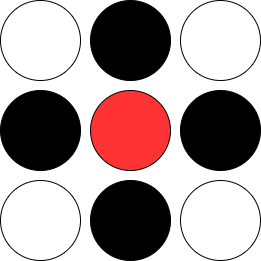
\includegraphics[width=0.5\textwidth, angle=0]{./fig/diagrams/neumann.png}
			\caption{von Neumann}
			\label{fig:neumann_neighbourhood}
		\end{subfigure}
    	&
		\begin{subfigure}[b]{0.2\textwidth}
			\centering
			
\includegraphics[width=0.5\textwidth, angle=0]{./fig/diagrams/moore.png}
			\caption{Moore}
			\label{fig:moore_neighbourhood}
		\end{subfigure}
    \end{tabular}
	\caption{Common neighbourhoods in discrete 2D environments of Agent-Based Simulation.}
	\label{fig:abs_neighbourhoods}
\end{center}
\end{figure}

We also implemented this spatial approach in Java using the well known ABS library RePast \cite{north_complex_2013}, to have a comparison with a state of the art approach and came to the same results as shown in Figure \ref{fig:sir_dunai}. This supports, that our pure functional approach can produce such results as well and compares positively to the state of the art in the ABS field.

\subsubsection{Implementation}
We start by defining the discrete 2D environment for which we use an indexed two dimensional array. Each cell stores the agent state of the last time-step, thus we use the \textit{SIRState} as type for our array data. Also, we re-define the agent signal function to take the structured environment \textit{SIREnv} as input instead of the list of all agents as in our previous approach. As output we keep the \textit{SIRState}, which is the state the agent is currently in. Also we run in the Random Monad as introduced before to avoid the random number correlation. 

\begin{HaskellCode}
type Disc2dCoord = (Int, Int)
type SIREnv      = Array Disc2dCoord SIRState

type SIRAgent g  = SF (Rand g) SIREnv SIRState
\end{HaskellCode}

Note that the environment is not returned as output because the agents do not directly manipulate the environment but only read from it. Again, this enforces the semantics of the \textit{parallel} update-strategy through the types where the agents can only see the previous state of the environment and see the actions of other agents reflected in the environment only in the next step.

Note that we could have chosen to use a StateT transformer with the \textit{SIREnv} as state, instead of passing it as input, with the agents then able to arbitrarily read/write, but this would have violated the semantics of our model because actions of agents would have become visible within the same time-step.

The implementation of the susceptible, infected and recovered agents are almost the same with only the neighbour querying now slightly different. 

Stepping the simulation needs a new approach because in each step we need to collect the agent outputs and update the environment for the next next step. For this we implemented a separate MSF, which receives the coordinates for every agent to be able to update the state in the environment after the agent was run. Note that we need use \textit{mapM} to run the agents because we are running now in the context of the Random Monad. This has the consequence that the agents are in fact run sequentially one after the other but because they cannot see the other agents actions nor observe changes in the shared read-only environment, it is \textit{conceptually} a \textit{parallel} update-strategy where agents run in lock-step, isolated from each other at conceptually the same time.
  
\begin{HaskellCode}
simulationStep :: RandomGen g => [(SIRAgent g, Disc2dCoord)]
               -> SIREnv -> SF (Rand g) () SIREnv
simulationStep sfsCoords env = MSF (\_ -> do
  let (sfs, coords) = unzip sfsCoords 
  -- run agents sequentially but with shared, read-only environment
  ret <- mapM (`unMSF` env) sfs
  -- construct new environment from all agent outputs for next step
  let (as, sfs') = unzip ret
      env' = foldr (\ (a, coord) envAcc -> updateCell coord a envAcc) 
               env (zip as coords)

      sfsCoords' = zip sfs' coords
      cont       = simulationStep sfsCoords' env'
  return (env', cont))
 
updateCell :: Disc2dCoord -> SIRState -> SIREnv -> SIREnv
\end{HaskellCode}

\subsubsection{Results}
We implemented rendering of the environments using the gloss library which allows us to cycle arbitrarily through the steps and inspect the spreading of the disease over time visually as seen in Figure \ref{fig:sir_dunai}.

\begin{figure}
\begin{center}
	\begin{tabular}{c c}
		\begin{subfigure}[b]{0.2\textwidth}
			\centering
			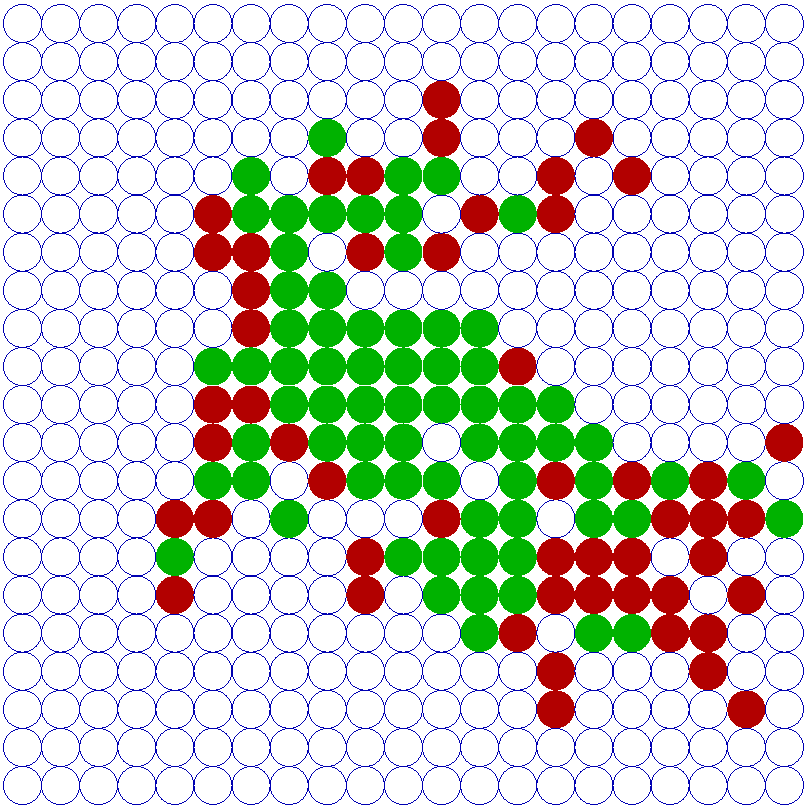
\includegraphics[width=1\textwidth, angle=0]{./fig/SIR_Dunai/SIR_Dunai_dt001_environment.png}
			\caption{Environment at $t = 50$}
			\label{fig:sir_dunai_env}
		\end{subfigure}
    	
    	&
  
		\begin{subfigure}[b]{0.23\textwidth}
			\centering
			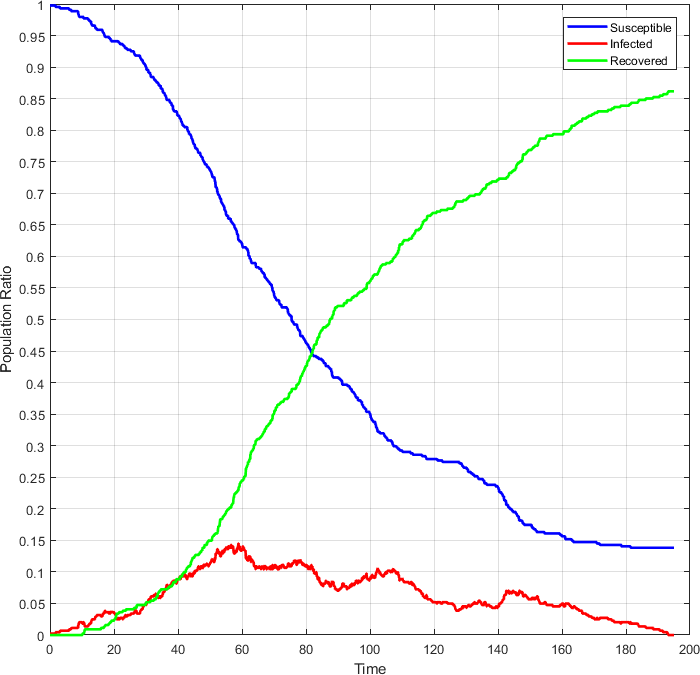
\includegraphics[width=1\textwidth, angle=0]{./fig/SIR_Dunai/SIR_Dunai_dt001.png}
			\caption{Dynamics over time}
			\label{fig:sir_dunai_env_dynamics}
		\end{subfigure}
	\end{tabular}
	
	\caption{Simulating the agent-based SIR model on a 21x21 2D grid with Moore neighbourhood (Figure \ref{fig:moore_neighbourhood}), a single infected agent at the center and same SIR parameters as in Figure \ref{fig:sir_sd_dynamics}. Simulation run until $t = 200$ with fixed $\Delta t = 0.01$. Last infected agent recovers around $t = 194$. The susceptible agents are rendered as blue hollow circles for better contrast.}
	\label{fig:sir_dunai}
\end{center}
\end{figure}

Note that the dynamics of the spatial SIR simulation which are seen in Figure \ref{fig:sir_dunai_env_dynamics} look quite different from the reference dynamics of Figure \ref{fig:sir_sd_dynamics}. This is due to a much more restricted neighbourhood which results in far fewer infected agents at a time and a lower number of recovered agents at the end of the epidemic, meaning that fewer agents got infected overall.

\subsubsection{Discussion}
By introducing a structured environment with a Moore neighbourhood, we showed the ABS ability to place the heterogeneous agents in a generic environment, which is the fundamental advantage of an agent-based approach over other simulation methodologies and allows us to simulate much more realistic scenarios.

Note, that an environment is not restricted to be a discrete 2D grid and can be anything from a continuous N-dimensional space to a complex network - one only needs to change the type of the environment and agent input and provide corresponding neighbourhood querying functions. 

\subsection{Additional Steps}
ABS involves a few more advanced concepts which we don't fully explore in this paper due to lack of space. Instead we give a short overview and discuss them without presenting code or going into technical details.

\subsubsection{Agent-Transactions}
Agent-transactions are necessary when an arbitrary number of interactions between two agents need to happen instantaneously without time-lag. The use-case for this are price negotiations between multiple agents where each pair of agents needs to come to an agreement in the same time-step \cite{epstein_growing_1996}. In object-oriented programming, the concept of synchronous communication between agents is implemented directly with method calls.

We have implemented synchronous interactions, which we termed agent-transactions in an additional step. We solved it pure functionally by running the signal functions of the transacting agent pair as often as their protocol requires but with $\Delta t=0$, which indicates the instantaneous character of agent-transactions.

\subsubsection{Event Scheduling}
Our approach is inherently time-driven where the system is sampled with fixed $\Delta t$. The other fundamental way to implement an ABS in general, is to follow an event-driven approach \cite{meyer_event-driven_2014}, which is based on the theory of Discrete Event Simulation \cite{zeigler_theory_2000}. In such an approach the system is not sampled in fixed $\Delta t$ but advanced as events occur where the system stays constant in between. Depending on the model, in an event-driven approach it may be more natural to express the requirements of the model.

In an additional step we have implemented a rudimentary event-driven approach, which allows the scheduling of events but had to omit it due to lack of space. Using the flexibility of MSFs we added a State transformer to the monad stack, which allows queuing of events into a priority queue. The simulation is advanced by processing the next event at the top of the queue, which means running the MSF of the agent which receives the event. The simulation terminates if there are either no more events in the queue or after a given number of events, or if the simulation time has advanced to some limit. Having made the transition to MSFs, implementing this feature was quite straight forward, which shows the power and strength of the generalised approach to FRP using MSFs.

\subsubsection{Dynamic Agent creation}
In the SIR model, the agent population stays constant - agents don't die and no agents are created during simulation - but some simulations \cite{epstein_growing_1996} require dynamic agent creation and destruction. We can easily add and remove agents signal functions in the recursive switch after each time-step. The only problem is that creating new agents requires unique agent ids but with the transition to MSFs we can add a monadic context, which allows agents to draw the next unique agent id when they create a new agent. 

\chapter{Dependent Types}
Independent of the programming paradigm, there exist fundamentally two approaches implementing agent-based simulation: time- and event-driven. In the time-driven approach, the simulation is stepped in fixed $\Delta t$ and all agents are executed at each time-step - they act virtually in lock-step at the same time. The approach is inspired by the theory of continuous system dynamics (TODO: cite).
In the event-driven approach, the system is advanced through events, generated by the agents, and the global system state changes by jumping from event to event, where the state is held constant in between. The approach is inspired by discrete event simulation (DES) (TODO: citation) which is formalized in the DEVS formalism \cite{zeigler_theory_2000}.

In a preceding paper we investigated how to derive a time-driven pure functional ABS approach in Haskell (TODO: cite my paper). We came to quite satisfactory results and implemented also a number of agent-based models of various complexity (TODO: cite schelling, sugarscape, agent zero). Still we identified weaknesses due to the underlying functional reactive programming (FRP) approach. It is possible to define partial implementations which diverge during runtime, which may be difficult to determine for complex models for a programmer at compile time. Also sampling the system with fixed $\Delta t$ can lead to severe performance problems when small $\Delta t$ are required, as was shown in our paper. The later problem is well known in the simulation community and thus as a remedy an event-driven approach was suggested \cite{meyer_event-driven_2014}.
In this paper for the first time, we derive a pure functional event-driven agent-based simulation. Instead of using Haskell, which provides already libraries for DES \cite{sorokin_aivika_2015}, we focus on the dependently typed pure functional programming language Idris. In our previous paper we hypothesised that dependent types may offer interesting new insights and approaches to ABS but it was unclear how exactly we can make use of them, which was left for further research. In this paper we hypothesise that, as opposed to a time-driven approach, the even-driven approach is especially suited to make proper use of dependent types due to its different nature. Note that both a pure functional event-driven approach to ABS \textit{and} the use of dependent types in ABS has so far never been investigated, which is the unique contribution of this paper.
If we can construct a dependently typed program of the SIR ABM which is total, then we have a proof-by-construction that the SIR model reaches a steady-state after finite time

Dependent Types are the holy grail in functional programming as they allow to express even stronger guarantees about the correctness of programs and go as far where programs and types become constructive proofs \cite{wadler_propositions_2015} which must be total by definition \cite{thompson_type_1991}, \cite{altenkirch_why_2005}, \cite{altenkirch_pi_sigma:_2010}, \cite{program_homotopy_2013}. Thus the next obvious step is to apply them to our pure functional approach of agent-based simulation. So far no research in applying dependent types to agent-based simulation exists at all and it is not clear whether dependent types do make sense in this setting. We explore this for the first time and ask more specifically how we can add dependent types to our pure functional approach, which conceptual implications this has for ABS and what we gain from doing so. Note that we can only scratch the surface and lay down basic ideas and leave a proper in-depth treatment of this topic for further research. We use Idris \cite{brady_idris_2013}, \cite{brady_type-driven_2017} as language of choice as it is very close to Haskell with focus on real-world application and running programs as opposed to other languages with dependent types e.g. Agda and Coq which serve primarily as proof assistants.

Dependent Types promise the following:

\begin{enumerate}
	\item Types as proofs - In dependently types languages, types can depend on any values and are first-class objects themselves. TODO: make more clear

	\item Totality and termination - Constructive proofs must terminate, this means a well-typed program (which is itself a proof) is always terminating which in turn means that it must consist out of total functions. A total function is defined by \cite{brady_type-driven_2017} as: it terminates with a well-typed result or produces a non-empty finite prefix of a well-typed infinite result in finite time. Idris is turing complete but is able to check the totality of a function under some circumstances but not in general as it would imply that it can solve the halting problem. Other dependently typed languages like Agda or Coq restrict recursion to ensure totality of all their functions - this makes them non turing complete.
\end{enumerate}

%An agent can be seen as a potentially infinite stream of continuations which at some point could return information to stop evaluating the next item of the stream which allows an agent to terminate.
%correspondence between temporal logics and FRP due to jeffery: is abs just another temporal logic?

%Ionesus talk on dependently typed programming in scientific computing
%https://www.pik-potsdam.de/members/ionescu/cezar-ifl2012-slides.pdf
%Ionescus talk on Increasingly Correct Scientific Computing
%https://www.cicm-conference.org/2012/slides/CezarIonescu.pdf
%Ionescus talk on Economic Equilibria in Type Theory
%https://www.pik-potsdam.de/members/ionescu/cezar-types11-slides.pdf
%Ionescus talk on Dependently-Typed Programming in Economic Modelling
%https://www.pik-potsdam.de/members/ionescu/ee-tt.pdf

dependent-types:
-> encode model-invariants on a meta-level
-> encode dynamics (what? feedbacks? positive/negative) on a meta-level
-> totality equals steady-state of a simulation, can enforce totality if required through type-level programming
-> probabilistic types can encode probability distributions in types already about which we can then reason
-> can we encode objectives in types?
-> agents as dependently typed continuations?: need a dependently typed concept of a process over time

\subsection{Related Work}
The authors of \cite{botta_functional_2011} are using functional programming as a specification for an agent-based model of exchange markets but leave the implementation for further research where they claim that it requires dependent types. This paper is the closest usage of dependent types in agent-based simulation we could find in the existing literature and to our best knowledge there exists no work on general concepts of implementing pure functional agent-based simulations with dependent types. As a remedy to having no related work to build on, we looked into works which apply dependent types to solve real world problems from which we then can draw inspiration from. 

The authors of \cite{brady_correct-by-construction_2010} use depend types to implement correct-by-construction concurrency in the Idris language \cite{brady_idris_2013}. They introduce the concept of a Embedded Domain Specific Language (EDSL) for concurrently locking/unlocking and reading/writing of resources and show that an implementation and formalisation are the same thing when using dependent types. We can draw inspiration from it by taking into consideration that we might develop a EDSL in a similar fashion for specifying general commands which agents can execute. The interpreter of such a EDSL can be pure itself and doesn't have to run in the IO Monad as our previous research (TODO: cite my PFE paper) has shown that ABS can be implemented pure.

In \cite{brady_idris_2011} the authors discuss systems programming with focus on network packet parsing with full dependent types in the Idris language \cite{brady_idris_2013}. Although they use an older version of it where a few features are now deprecated, they follow the same approach as in the previous paper of constructing an EDSL and and writing an interpreter for the EDSL. In a longer introduction of Idris the authors discus its ability for termination checking in case that recursive calls have an argument which is structurally smaller than the input argument in the same position and that these arguments belong to a strictly positive data type. We are particularly interested in whether we can implement an agent-based simulation which termination can be checked at compile time - it is total.

In \cite{brady_programming_2013} the author discusses programming and reasoning with algebraic effects and dependent types in the Idris language \cite{brady_idris_2013}. They claim that monads do not compose very well as monad transformer can quickly become unwieldy when there are lots of effects to manage. As a remedy they propose algebraic effects and implement them in Idris and show how dependent types can be used to reason about states in effectful programs. In our previous research (TODO: cite my PFE paper) we relied heavily on Monads and transformer stacks and we indeed also experienced the difficulty when using them. Algebraic effects might be a promising alternative for handling state as the global environment in which the agents live or threading of random-numbers through the simulation which is of fundamental importance in ABS. Unfortunately algebraic effects cannot express continuations (according to the authors of the paper) which is but of fundamental importance for pure functional ABS as agents are on the lowest level built on continuations - synchronous agent interactions and time-stepping builds directly on continuations. Thus we need to find a different representation of agents - GADTs seem to be a natural choice as all examples build heavily on them and they are very flexible.

In \cite{fowler_dependent_2014} the authors apply dependent types to achieve safe and secure web programming. This paper shows how to implement dependent effects, which we might draw inspiration from of how to implement agent-interactions which, depending on their kind, are effectful e.g. agent-transactions or events.

In \cite{brady_state_2016} the author introduces the ST library in Idris, which allows a new way of implementing dependently typed state machines and compose them vertically (implementing a state machine in terms of others) and horizontally (using multiple state machines within a function). In addition this approach allows to manage stateful resources e.g. create new ones, delete existing ones. We can draw further inspiration from that approach on how to implement dependently typed state machines, especially composing them hierarchically, which is a common use case in agent-based models where agents behaviour is modelled through hierarchical state-machines. As with the Algebraic Effects, this approach doesn't support continuations (TODO: is this so?), so it is not really an option to build our architecture for our agents on it, but it may be used internally to implement agents or other parts of the system. What we definitely can draw inspiration from is the implementation of the indexed Monad \textit{STrans} which is the main building block for the ST library.

The book \cite{brady_type-driven_2017} is a great source to learn pure functional dependently typed programming and in the advanced chapters introduces the fundamental concepts of dependent state machine and dependently typed concurrent programming on a simpler level than the papers above. One chapter discusses on how to implement a messaging protocol for concurrent programming, something we can draw inspiration from for implementing our synchronous agent interaction protocols.

The authors of \cite{sculthorpe_safe_2009} apply dependent types to FRP to avoid some run-time errors and implement a dependently typed version of the Yampa library in Agda. FRP was the underlying concept of implementing agent-based model we took on in our previous approach (TODO: cite). We could have taken the same route and lift FRP into dependent types but we chose explicitly to not go into this direction and look into complementing approaches on how to implement agent-based models.

The fundamental difference to all these real-world examples is that in our approach, the system evolves over time and agents act over time. A fundamental question will be how we encode the monotonous increasing flow of time in types and how we can reflect in the types that agents act over time.

%The authors of \cite{ionescu_dependently-typed_2012} discuss how to use dependent types to specify fundamental theorems of economics, unfortunately they are not computable and thus not constructive, thus leaving it more to a theoretical, specification side.
%Ionesus talk on dependently typed programming in scientific computing
%https://www.pik-potsdam.de/members/ionescu/cezar-ifl2012-slides.pdf
%Ionescus talk on Increasingly Correct Scientific Computing
%%https://www.cicm-conference.org/2012/slides/CezarIonescu.pdf
%Ionescus talk on Economic Equilibria in Type Theory
%https://www.pik-potsdam.de/members/ionescu/cezar-types11-slides.pdf
%Ionescus talk on Dependently-Typed Programming in Economic Modelling
%https://www.pik-potsdam.de/members/ionescu/ee-tt.pdf

\section{Concepts of Dependent Types in Agent-Based Simulation}
Independent of the programming paradigm, there exist fundamentally two approaches implementing agent-based simulation: time- and event-driven. In the time-driven approach, the simulation is stepped in fixed $\Delta t$ and all agents are executed at each time-step - they act virtually in lock-step at the same time. The approach is inspired by the theory of continuous system dynamics (TODO: cite).
In the event-driven approach, the system is advanced through events, generated by the agents, and the global system state changes by jumping from event to event, where the state is held constant in between. The approach is inspired by discrete event simulation (DES) (TODO: citation) which is formalized in the DEVS formalism \cite{zeigler_theory_2000}.

In a preceding paper we investigated how to derive a time-driven pure functional ABS approach in Haskell (TODO: cite my paper). We came to quite satisfactory results and implemented also a number of agent-based models of various complexity (TODO: cite schelling, sugarscape, agent zero). Still we identified weaknesses due to the underlying functional reactive programming (FRP) approach. It is possible to define partial implementations which diverge during runtime, which may be difficult to determine for complex models for a programmer at compile time. Also sampling the system with fixed $\Delta t$ can lead to severe performance problems when small $\Delta t$ are required, as was shown in our paper. The later problem is well known in the simulation community and thus as a remedy an event-driven approach was suggested \cite{meyer_event-driven_2014}.
In this paper for the first time, we derive a pure functional event-driven agent-based simulation. Instead of using Haskell, which provides already libraries for DES \cite{sorokin_aivika_2015}, we focus on the dependently typed pure functional programming language Idris. In our previous paper we hypothesised that dependent types may offer interesting new insights and approaches to ABS but it was unclear how exactly we can make use of them, which was left for further research. In this paper we hypothesise that, as opposed to a time-driven approach, the even-driven approach is especially suited to make proper use of dependent types due to its different nature. Note that both a pure functional event-driven approach to ABS \textit{and} the use of dependent types in ABS has so far never been investigated, which is the unique contribution of this paper.
If we can construct a dependently typed program of the SIR ABM which is total, then we have a proof-by-construction that the SIR model reaches a steady-state after finite time

Dependent Types are the holy grail in functional programming as they allow to express even stronger guarantees about the correctness of programs and go as far where programs and types become constructive proofs \cite{wadler_propositions_2015} which must be total by definition \cite{thompson_type_1991}, \cite{altenkirch_why_2005}, \cite{altenkirch_pi_sigma:_2010}, \cite{program_homotopy_2013}. Thus the next obvious step is to apply them to our pure functional approach of agent-based simulation. So far no research in applying dependent types to agent-based simulation exists at all and it is not clear whether dependent types do make sense in this setting. We explore this for the first time and ask more specifically how we can add dependent types to our pure functional approach, which conceptual implications this has for ABS and what we gain from doing so. Note that we can only scratch the surface and lay down basic ideas and leave a proper in-depth treatment of this topic for further research. We use Idris \cite{brady_idris_2013}, \cite{brady_type-driven_2017} as language of choice as it is very close to Haskell with focus on real-world application and running programs as opposed to other languages with dependent types e.g. Agda and Coq which serve primarily as proof assistants.

Dependent Types promise the following:

\begin{enumerate}
	\item Types as proofs - In dependently types languages, types can depend on any values and are first-class objects themselves. TODO: make more clear

	\item Totality and termination - Constructive proofs must terminate, this means a well-typed program (which is itself a proof) is always terminating which in turn means that it must consist out of total functions. A total function is defined by \cite{brady_type-driven_2017} as: it terminates with a well-typed result or produces a non-empty finite prefix of a well-typed infinite result in finite time. Idris is turing complete but is able to check the totality of a function under some circumstances but not in general as it would imply that it can solve the halting problem. Other dependently typed languages like Agda or Coq restrict recursion to ensure totality of all their functions - this makes them non turing complete.
\end{enumerate}

%An agent can be seen as a potentially infinite stream of continuations which at some point could return information to stop evaluating the next item of the stream which allows an agent to terminate.
%correspondence between temporal logics and FRP due to jeffery: is abs just another temporal logic?

dependent-types:
-> encode model-invariants on a meta-level
-> encode dynamics (what? feedbacks? positive/negative) on a meta-level
-> totality equals steady-state of a simulation, can enforce totality if required through type-level programming
-> probabilistic types can encode probability distributions in types already about which we can then reason
-> can we encode objectives in types?
-> agents as dependently typed continuations?: need a dependently typed concept of a process over time

As shown in our previous research (TODO: cite), the strong static type system of Haskell allows us to guarantee a lot already at compile time:
\begin{itemize}
	\item Purity - no side-effects possible at all 
	\item Monad - controlled, explicit side-effects possible
	\item generic types allow to guarantee for all
\end{itemize}

Dependent Types in Idris bring the strong static type system of Haskell to a new level, which allows us to both guarantee more things at compile time and express things through type-level computations. This means the following at compile time

\begin{itemize}
	\item Ruling out ever larger classes of bugs
	\item Dependent State Machines
	\item Dependent Agent Interactions
	\item Flow Of Time
	\item Totality
	\item Constructive Proofs
\end{itemize}

\subsection{Ruling out Bugs}
\begin{enumerate}
	\item Index out of bounds access of Lists and Vectors can be guaranteed not to happen any more when using proofs of existence of the element in the list or vector.
	\item Size of list or vector stays constant / increases / decreases / sum of length of multiple vectors guaranteed to be of some number
\end{enumerate}

The question is how far we can generalise our approaches because we fear that the downside of using dependently typed abs is that every implementation needs to start from Scratch: we cant write a general library for it like chimera because the more we put into types, the more specific it is => individual implementation which reuses existing 'patterns' like state machines, messages,...

\subsection{General Agent Interface}
using dependent types to specify the general commands available for an agent. here we can follow the approach of an DSEL as described in \cite{brady_correct-by-construction_2010} and write then an interpreter for it. It is of importance that the interpreter shall be pure itself and does not make use of any fancy IO stuff.

\subsection{Dependent State Machines}
dependent state machines in abs for internal state because that is very Common in ABS. Here we can draw inspiration from the paper \cite{brady_state_2016} and book \cite{brady_type-driven_2017}.

\subsection{Environment}
One of the main advantages of Agent-Based Simulation over other simulation methods e.g. System Dynamics is that agents can live within an environment. Many agent-based models place their agents within a 2D discrete NxM environment where agents either stay always on the same cell or can move freely within the environment where a cell has 0, 1 or many occupants. Ultimately this boils down to accessing a NxM matrix represented by arrays or a similar data structure. In imperative languages accessing memory always implies the danger of out-of-bounds exceptions \textit{at run-time}. With dependent types we can represent such a 2d environment using vectors which carry their length in the type (TODO: discuss them in background) thus fixing the dimensions of such a 2D discrete environment in the types. This means that there is no need to drag those bounds around explicitly as data. Also by using dependent types like Fin which depend on the dimensions we can enforce at compile time that we can only access the data structure within bounds. If we want to we can also enforce in the types that the environment will never be an empty one where N, M > 0.

\begin{minted}{haskell}
Disc2dEnv : (w : Nat) -> (h : Nat) -> (e : Type) -> Type
Disc2dEnv w h e = Vect (S w) (Vect (S h) e)

data Disc2dCoords : (w : Nat) -> (h : Nat) -> Type where
  MkDisc2dCoords : Fin (S w) -> Fin (S h) -> Disc2dCoords w h
  
centreCoords : Disc2dEnv w h e -> Disc2dCoords w h
centreCoords {w} {h} _ =
    let x = halfNatToFin w
        y = halfNatToFin h
    in  mkDisc2dCoords x y
  where
    halfNatToFin : (x : Nat) -> Fin (S x)
    halfNatToFin x = 
      let xh   = divNatNZ x 2 SIsNotZ 
          mfin = natToFin xh (S x)
      in  fromMaybe FZ mfin
      
setCell :  Disc2dCoords w h
        -> (elem : e)
        -> Disc2dEnv w h e
        -> Disc2dEnv w h e
setCell (MkDisc2dCoords colIdx rowIdx) elem env 
    = updateAt colIdx (\col => updateAt rowIdx (const elem) col) env
 
getCell :  Disc2dCoords w h
        -> Disc2dEnv w h e
        -> e
getCell (MkDisc2dCoords colIdx rowIdx) env
    = index rowIdx (index colIdx env)
    
neumann : Vect 4 (Integer, Integer)
neumann = [         (0,  1), 
           (-1,  0),         (1,  0),
                    (0, -1)]

moore : Vect 8 (Integer, Integer)
moore = [(-1,  1), (0,  1), (1,  1),
         (-1,  0),          (1,  0),
         (-1, -1), (0, -1), (1, -1)]

-- TODO: can we express that n <= len?
filterNeighbourhood :  Disc2dCoords w h
                    -> Vect len (Integer, Integer)
                    -> Disc2dEnv w h e 
                    -> (n ** Vect n (Disc2dCoords w h, e))
filterNeighbourhood {w} {h} (MkDisc2dCoords x y) ns env =
    let xi = finToInteger x
        yi = finToInteger y
    in  filterNeighbourhood' xi yi ns env
  where
    filterNeighbourhood' :  (xi : Integer)
                         -> (yi : Integer)
                         -> Vect len (Integer, Integer)
                         -> Disc2dEnv w h e 
                         -> (n ** Vect n (Disc2dCoords w h, e))
    filterNeighbourhood' _ _ [] env = (0 ** [])
    filterNeighbourhood' xi yi ((xDelta, yDelta) :: cs) env 
      = let xd = xi - xDelta
            yd = yi - yDelta
            mx = integerToFin xd (S w)
            my = integerToFin yd (S h)
        in case mx of
            Nothing => filterNeighbourhood' xi yi cs env 
            Just x  => (case my of 
                        Nothing => filterNeighbourhood' xi yi cs env 
                        Just y  => let coord      = MkDisc2dCoords x y
                                       c          = getCell coord env
                                       (_ ** ret) = filterNeighbourhood' xi yi cs env
                                   in  (_ ** ((coord, c) :: ret)))
\end{minted}

\subsection{Dependent Agent Interactions}
\subsubsection{Agent Transactions}
dependently typed message protocols in ABS because its very common, and easily done thorugh methods in OOP: sugarscape mating and trading protocol
using a DSEL \cite{brady_correct-by-construction_2010} to restrict the available primitives in the message protocol?

\subsubsection{Data Flow}
TODO: can dependent types be used in the Data Flow Mechanism?
\subsubsection{Event Scheduling}
TODO: can dependent types be used in the event-scheduling mechanism?

\subsection{Flow Of Time}
TODO: can dependent types be used to express the flow of time and its strongly monotonic increasing?

\subsection{Totality}
totality of parts or the whole simulation e.g. in case of the SIR model we can informally reason that the simulation MUST reach an equilibrium (a steady state from which there is no escape: the dynamics wont't change anymore, derivations are 0) after a finite number of steps. if we can construct a total program which expresses this, we have a formal proof of that which is 1) a specification of the model 2) generates the dynamics 3) is a proof that it reaches equilibrium

\subsection{Constructive Proofs}
- An agent-based model and the simulated dynamics of it is itself a constructive proof which explain a real-world phenomenon sufficiently good
- proof of the existence of an agent: holds always only for the current time-step or for all time, depending on the model. e.g. in the SIR model no agents are removed from / added to the system thus a proof holds for all time. In sugarscape agents are removed / added dynamically so a proof might become invalid after a time or one can construct a proof only from a given time on e.g. when one wants to prove that agent X exists but agent X is only created at time t then before time t the prove cannot be constructed and is uninhabited and only inhabited from time t on.

\section{Dependently Typed SIR}
Intuitively, based upon our model and the equations we can argue that the SIR model enters a steady state as soon as there are no more infected agents. Thus we can informally argue that a SIR model must always terminate as:
\begin{enumerate}
	\item Only infected agents can infect susceptible agents.
	\item Eventually after a finite time every infected agent will recover.
	\item There is no way to move from the consuming \textit{recovered} state back into the \textit{infected} or \textit{susceptible} state \footnote{There exists an extended SIR model, called SIRS which adds a cycle to the state-machine by introducing a transition from recovered to susceptible but we don't consider that here.}.
\end{enumerate}

Thus a SIR model must enter a steady state after finite steps / in finite time. 

This result gives us the confidence, that the agent-based approach will terminate, given it is really a correct implementation of the SD model. Still this does not proof that the agent-based approach itself will terminate and so far no proof of the totality of it was given. Dependent Types and Idris ability for totality and termination checking should theoretically allow us to proof that an agent-based SIR implementation terminates after finite time: if an implementation of the agent-based SIR model in Idris is total it is a proof by construction. Note that such an implementation should not run for a limited virtual time but run unrestricted of the time and the simulation should terminate as soon as there are no more infected agents. We hypothesize that it should be possible due to the nature of the state transitions where there are no cycles and that all infected agents will eventually reach the recovered state. 
Abandoning the FRP approach and starting fresh, the question is how we implement a \textit{total} agent-based SIR model in Idris. Note that in the SIR model an agent is in the end just a state-machine thus the model consists of communicating / interacting state-machines. In the book \cite{brady_type-driven_2017} the author discusses using dependent types for implementing type-safe state-machines, so we investigate if and how we can apply this to our model. We face the following questions: how can we be total? can we even be total when drawing random-numbers? Also a fundamental question we need to solve then is how we represent time: can we get both the time-semantics of the FRP approach of Haskell AND the type-dependent expressivity or will there be a trade-off between the two?

-- TODO: express in the types
-- SUSCEPTIBLE: MAY become infected when making contact with another agent
-- INFECTED:    WILL recover after a finite number of time-steps
-- RECOVERED:   STAYS recovered all the time

-- SIMULATION:  advanced in steps, time represented as Nat, as real numbers are not constructive and we want to be total
--              terminates when there are no more INFECTED agents


show formally that abs does resemble the sd approach: need an idea of a proof and then implement it in dependent types: look at 3 agent system: 2 susceptible, 1 infected. or maybe 2 agents only

%A susceptible agent can only become infected when it comes into contact with an infected agent. The probability of a susceptible agent making contact with an infected one is naturally (number of infected agents) / (total number of agents). For the infection to occur we multiply the contact with the infectivity parameter \Gamma. A susceptible agent makes on average \Beta contacts per time-unit. This results in the following formula:
%
%\begin{align}
%prob &= \frac{I \beta \gamma}{N} \\
%\end{align}
%
%This is for a single agent, which we then need to multiply by the number of susceptible agents because all of them make contact.
%
%TODO: implement sir with state-machine approach from Idris. an idea would be to let infected agents generate infection- actions: the more infected agents the more infection-actions => zero infected agents mean zero infection actions. this list can then be reduced?
%
%can we also emulate SD in Idris and formulate positive/negative feedback loops in types?

\subsection{A constructive proof of totality}
The idea is to implement a total agent-based SIR simulation, where the termination does NOT depend on time (is not terminated after a finite number of time-steps, which would be trivial). The dynamics of the system-dynamics SIR model are in equilibrium (won't change anymore) when the infected stock is 0. This can (probably) be shown formally but intuitionistic it is clear because only infected agents can lead to infections of susceptible agents which then make the transition to recovered after having gone through the infection phase. Thus an agent-based implementation of the SIR simulation has to terminate if it is implemented correctly because all infected agents will recover after a finite number of steps after then the dynamics will be in equilibrium.
Thus we need to 'tell' the type-checker the following:
1) no more infected agents is the termination criterion
2) all infected agents will recover after a finite number of time => the simulation will eventually run out of infected agents But when we look at the SIR+S model we have the same termination criterion, but we cannot guarantee that it will run out of infected => we need additional criteria
3) infected agents are 'generated' by susceptible agents
4) susceptible agents are NOT INCREASING (e.g. recovered agents do NOT turn back into susceptibles)
Interesting: can we adopt our solution (if we find it), into a SIRS	implementation? this should then break totality. also how difficult is it?

The HOTT book states that lists, trees,... are inductive types/inductively defined structures where each of them is characterized by a corresponding "induction principle". For a proof of totality of SIR we need to find the "induction principle" of the SIR model and implement it. What is the inductive, defining structure of the SIR model? is it a tree where a path through the tree is one simulation dynamics? or is it something else? it seems that such a tree would grow and then shrink again e.g. infected agents. Can we then apply this further to (agent-based) simulation in general?

TODO: \url{https://stackoverflow.com/questions/19642921/assisting-agdas-termination-checker/39591118}

\section{Constructivism}
TODO: ABS is constructive: "if you can't grow it, you can't explain it" (epstein)
TODO: Dependent Types are constructive
=> there are no excluded middle in both approaches
=> are there deeper, philosophical connections going on? does it have even deeper implications?
TODO: shortly discuss Propositions as types from HOTT 1.11. In the end a dependently typed ABS is then a constructive proof of WHAT? the model? if we have a total SIR implementation its a constructive proof that the agent-based implementation is total / will reach an equilibrium after a finite number of steps. Still it is not entirely clear WHAT WE ARE PROVING when we are constructing dependently typed agent-based simulations. I need to think about this more carefully
TODO: checkout my notes in 1st annual review on constructivism / popper 

Law of excluded middle does not hold anymore because it would require us to be able to effectively compute / decide whether a proposition is true or false - which amounts to solving the halting problem, which is not possible in the general case.

\section{Related Research}
Already noted in the Introduction, \cite{huberman_evolutionary_1993} where the first to discuss the differences update-strategies can make and introduced the terms of synchronous and asynchronous updates. They define to be synchronous as agents being updated in unison and asynchronous where one agent is updated and the others are held constant.

\medskip

\cite{a_framework_2008} give an approach for ABS on GPUs which is a very different approach to updating and iterating agents in ABS. They discuss execution order at length, highlight the problem of inducing a specific execution-order in a model which is problematic for parallel execution and give solutions how to circumvent these shortcomings. Although we haven't mapped our ideas to GPUs we explicitly include an approach for data-parallelism which, we hypothesize, can be utilized to roughly map their approach onto our terminology. 
	
\medskip
	
\cite{botta_time_2010} sketch a minimal ABS implementation in Haskell which is very similar in the basic structure of ours. This proves that our approach seems to be a very natural one to apply to Haskell. Their focus is primarily on economic simulations and instead of iterating a simulation with a global time, their focus is on how to synchronize agents which have internal, local transition times. Although their work uses Haskell as well, our focus is very different from theirs and approaches ABS in a more general and comprehensive way.

\medskip

\cite{dawson_opening_2014} describe basic inner workings of ABS environments and compare their implementation in C++ to the existing ABS environment AnyLogic which is programmed in Java. They explicitly mention asynchronous and synchronous time-models and compare them in theory but unfortunately couldn't report the results of asynchronous updates due to limited space. They interpret asynchronous time-models to be the ones in which an agent acts at random time intervals and synchronous time-models where agents are updated all in same time intervals.

\medskip

\cite{yuxuan_agent-based_2016} presents in his Master-Thesis a comprehensive discussion on how to implement an ABS for state-charts in Java and also mentions synchronous and asynchronous time-models. He identifies the asynchronous time-model to be one in which updates are triggered by the exchange of messages and the synchronous ones which trigger changes immediately without the indirection of messages.

\medskip

We observe that there seems to be a variety of meanings attributed to the terminology of asynchronous and synchronous updates but the very semantic and technical details are unclear and not described very precisely. In the next section we will address this issue by presenting the basic background and propose properties for a new terminology from which we can derive common update-strategies.

\section{Conclusion and further research}

So far we only looked at recursive simulation in a simulation with a strictly sequential update-strategy where agents are updated in sequence after each other as defined in TODO: cite my Art-Of-Iteration Paper. We leave the question of how Meta-ABS would apply to the parallel update-strategy and whether it is reasonable to extend it to that strategy or not for further research.

Research Questions
\begin{enumerate}
	\item How does deep regression influence the dynamics of a system? Hypothesis: TODO
	\item How do the dynamics of a system change when using perfect information or learning local information? Hypothesis: TODO
	\item Is a hidden markov model suitable for the local learning? Hypothesis: TODO
	\item How can MetaABS best be implemented? Hypothesis: implementing a MetaABS EDSL in a pure functional language like Haskell, should be best suited due to its inherent recursive, declarative nature, which should allow a direct mapping of features of this paradigm to the specification of the meta-model
\end{enumerate}

Problems
\begin{itemize}
	\item Definition of a recursive, declarative description of the Model.
	\item Perfect information about other agents is not realistic and runs counter to agent-based simulation (especially in social sciences) thus an Agent needs to be able to have local, noisy representations of the other agents.
	\item Local representation of other agents could be captured by Hidden Markov Models: observe what other agents do but have hidden interpretation of their internal state - these internal state-representations can be different between the local and the global version whereas the agent learns to represent the global version as best as possible locally.
	\item Infinite regress is theoretically possible but not on computers, we need to terminate at some point
\end{itemize}

\begin{acks}
The authors would like to thank I. Perez, H. Nilsson, J. Greensmith, T. Schwarz and H. Vollbrecht for constructive comments and valuable discussions.
\end{acks}

% Bibliography
%\bibliographystyle{../../../templates/IEEEtran/bibtex/IEEEtran}
\bibliographystyle{../../templates/acmart/ACM-Reference-Format}
\bibliography{../../../references/phdReferences.bib}

\end{document}